\section{Clasificaci�n}
\label{clasificacion}

\subsection{Vecinos m�s cercanos - kNN}
\subsubsection{Distancia euclidiana}
\subsubsection{Distancia de hamming}
\subsubsection{Distancia mahalanobis}


\subsection{Support Vector Machine - SVM}

Las m�quinas de vectores de soporte (Support Vector Machines, SVMs) es una reciente t�cnica de aprendizaje supervisado desarrollado por \cite{SVM, SVM2}. SVM ha sido aplicado exitosamente a un gran n�mero de problemas de clasificaci�n.

Como ejemplo introductorio, suponga un problema de clasificaci�n separable en un espacio de dimensi�n~$2$. Hay muchos hiperplanos que pueden separar las dos clases de datos, ver figura~\ref{fig:svm_1}-(a).
\begin{figure}[!htbp]
    \centering
    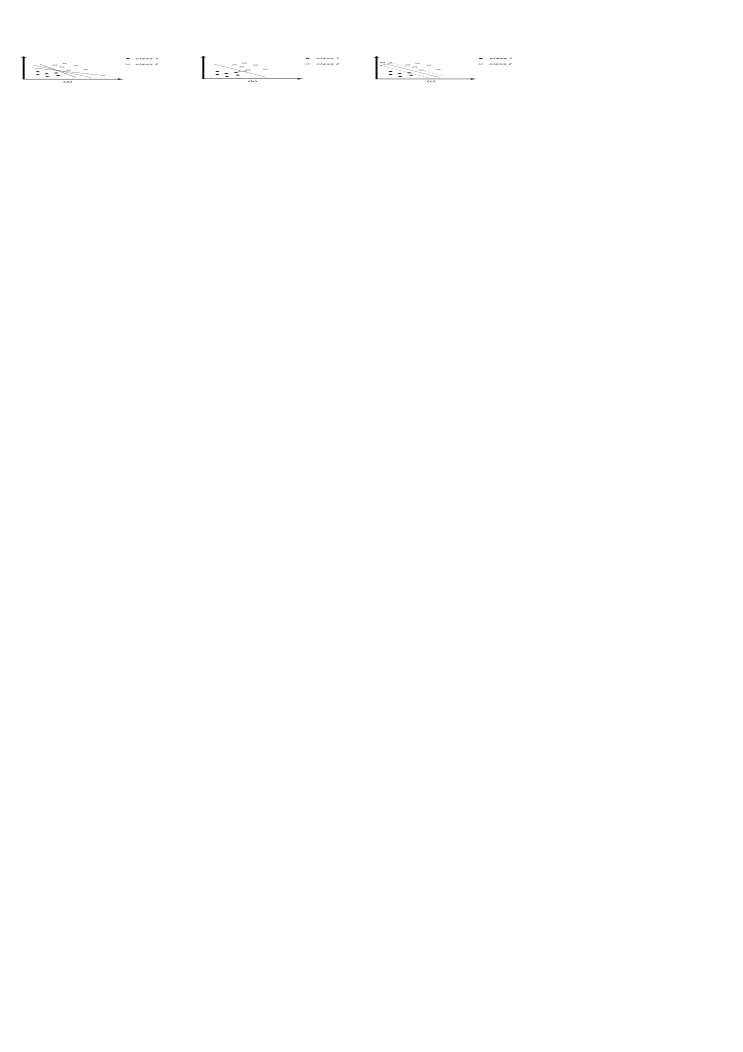
\includegraphics[scale=0.8]{imagen/svm_1.pdf}
    \caption{(a) Posibles hiperplanos; (b) selecci�n de un �nico hiperplano que maximiza la distancia de los puntos m�s cercanos de cada clase; (c) hiperplano de separaci�n �ptimo que maximiza el margen.}
    \label{fig:svm_1}
\end{figure}

Suponga un hiperplano tal que los puntos $x$ que se encuentren en el hiperplano satisfacen,
\begin{align}
\label{eq:hiperplano}
\omega^Tx+b &= 0
\end{align}
donde $\omega$ es la normal del hiperplano, $|b|/\|\omega\|$ es la distancia perpendicular desde el hiperplano al origen, y $\|\omega\|$ es la norma Euclidiana de $\omega$.

Definiendo \textit{\textbf{margen}} (M) como la suma de las distancias entre este hiperplano y los puntos m�s cercanos de cada clase, figura~\ref{fig:svm_1}-(b); el hiperplano de separaci�n ser� �ptimo si �ste maximiza dicho margen, figura~\ref{fig:svm_1}-(c).


\subsubsection{SVM lineal}
Si tenemos un conjunto de entrenamiento $\mathcal{D}$ de la forma,
\begin{align*}
\mathcal{D} & = \left\{ (\mathbf{x}_i, y_i)\mid\mathbf{x}_i \in \mathbb{R}^p,\, y_i \in \{-1,1\}\right\}_{i=1}^n
\end{align*}
donde $y_i$ es $-1$ o $1$, indicando la clase a la cual pertenece el punto $x_i$. se desea encontrar en~\refEQ{eq:hiperplano} los $w$ y $b$ que maximicen el margen, sujeto a las siguientes restricciones,
\begin{align*}
\omega^Tx_k-b &\geq~ ~ ~1, \hspace*{1.5cm} \mbox{for} \hspace{1mm} y_k=~ ~ ~1\\
\omega^Tx_k-b &\leq-1, \hspace*{1.5cm} \mbox{for} \hspace{1mm} y_k=-1
\end{align*}
Estas ecuaciones pueden combinarse con el siguiente conjunto de inecuaciones,
\begin{align}
\label{eq:svm}
y_k(\omega^Tx_k-b)-1\geq0, \hspace{3mm} k=1,...,n.
\end{align}

Notar que si $\mathcal{D}$ es linealmente separable, se pueden seleccionar dos hiperplanos de tal manera que no hay puntos entre ellos maximizando sus distancias, ver figura \ref{fig:Svm_max_sep_hyperplane_with_margin}. Estos hiperplanos pueden describirse como: $\omega^Tx_k-b=1$ y $\omega^Tx_k-b=-1$, seg�n los $x_k$ correspondan a la clase~$1$ �~$-1$, respectivamente. Y las distancias al origen de los hiperplanos son: $\frac{|b-1|}{\|\omega\|}$ y $\frac{|b+1|}{\|\omega\|}$, respectivamente. Entonces, el margen M es igual a $2/\|\omega\|$ y el problema es resulto minimizando $\|w\|$ sujeto a \refEQ{eq:svm}.
\begin{figure}[!htbp]
    \centering
    \includegraphics[scale=0.25]{imagen/Svm_max_sep_hyperplane_with_margin.png}
    \caption{M�rgenes para un SVM entrenado con datos de dos clases. Las vectores en los m�rgenes son llamados \textit{\textbf{vectores soportes}}}
    \label{fig:Svm_max_sep_hyperplane_with_margin}
\end{figure}


Idealmente, el modelo basado en SVM deber�a producir un hiperplano que separe completamente los datos en dos categor�as. Sin embargo, una separaci�n perfecta no siempre es posible, ver figura \ref{fig:nonsep}.
\begin{figure}[!htbp]
    \centering
    \includegraphics[scale=0.8]{imagen/svm_2.pdf}
    \caption{Problema de clasificaci�n no separable}
    \label{fig:nonsep}
\end{figure}

En estos casos, son a�adidas $\xi_k$ (\textit{slack variables}) en la formulaci�n del problema con el objetivo de relajar las restricciones. Luego, el conjunto de inecuaciones toman la siguiente forma,
\begin{align*}
% \label{eq:svm3}
y_k(\omega^Tx_k-b)\geq1-\xi_k, \hspace{3mm} k=1,...,n .
\end{align*}


La funci�n objetivo es entonces incrementada por una funci�n que penaliza los $\xi_k$ que no son cero. La optimizaci�n se vuelve un balance entre tener gran margen y penalizaci�n de errores,
\begin{align*}
\min_{\mathbf{w},\mathbf{\xi}, b } \left\{\frac{1}{2} \|\mathbf{w}\|^2 + C \sum_{k=1}^n \xi_k \right\}
\end{align*}
sujeto a,
\begin{align*}
y_k(\omega^Tx_k-b) & \geq1-\xi_k, \hspace{3mm} k=1,...,n .\\
\xi_k & \ge 0
\end{align*}
donce C que controla la compensaci�n entre errores de entrenamiento y los m�rgenes r�gidos, creando as� un margen blando (\textit{soft margin}) que permita algunos errores en la clasificaci�n a la vez que los penaliza.

\subsubsection{SVM no lineal - Kernels}

% The extension from the linear to the nonlinear case is straightforward.
% The linear separating hyperplane is calculated in a higher dimensional feature space where the input data lie after being mapped by a nonlinear mapping $\varphi(x)$. Then, the classifier in the case of nonlinear data can be written as
% \begin{equation} \label{eq:svm4}
% y_k[\omega^T\varphi(x_k)+b]\geq1-\xi_k, \hspace{3mm} k=1,...,n .
% \end{equation}
% Taking into account the Lagrangian formulation of the problem, the training data only appear in the form of dot products between their nonlinear mapping, {\em i.e.}, they appear as $\varphi(x_k)^T\varphi(x_\ell)$ $\forall k,\ell$. Then, no explicit construction of the nonlinear mapping $\varphi(x)$ is needed, by applying the so-called kernel trick. That is, by defining a Kernel as $K(x_k,x_\ell)=\varphi(x_k)^T\varphi(x_\ell)$ for $k,\ell=1,...,n$.
% 
% Finally, the SVM solution can be found by solving the following optimization problem
% \begin{eqnarray} \label{eq:svm5}
% \min_{\omega,b,\xi}  &  J_P(\omega,\xi)=\frac{1}{2}\omega^T\omega+c \sum_{k=1}^n \xi_k
% \\
% \mbox{s.t.}  &  y_k[\omega^T\varphi(x_k)+b]  \geq  1-\xi_k, & k=1,...,n\nonumber
% \\
%   &  \xi_k  \geq  0, &  k=1,...,n.\nonumber
% \end{eqnarray}
% 
% Resorting to the dual of problem (\ref{eq:svm5}), the solution of the Quadratic Programming (QP) problem is the set of the real positive constants $\alpha_k$, and the SVM classifier takes the following form
% \begin{equation} \label{eq:svm7}
% y(x)=sign[\sum_{k=1}^n\alpha_ky_kK(x,x_k)+b] .
% \end{equation}
% 
% Different Kernels have been used in the literature to solve pattern recognition problems. Linear, Polynomial and Radial Basis Functions (RBF) Kernels are among the most popular in the bibliography and they are respectively defined as follows
% %The real positive constants $\alpha_k$ are the solution of the quadratic programming (QP) problem , that makes the nonlinear SVM classifier to take the form of (\ref{eq:svm7}).
% \begin{eqnarray*}
% K_{linear}(x_k,x_\ell) & = & x_k^Tx_\ell ,\\
% K_{polynomial}(x_k,x_\ell) & = & (1+x_k^Tx_\ell)^d ,\nonumber \\
% K_{RBF}(x_k,x_\ell) & = & exp(-\parallel x_k-x_\ell \parallel_2^2/\sigma^2) .\nonumber
% \end{eqnarray*}
% 
% %Support Vector Machines is a quite recent technique of statistical learning theory developed by Vapnik (\cite{Vapnik_1995}, \cite{Vapnik_1998}).
% %In recent years, SVM has been successfully applied to a large number of classification problems.
% %Particularly, SVM-based classifiers have shown a promising performance in Automatic Signature Verification as \cite{Justino_et_al_2004} and \cite{Ozgunduz_et_al_2005} demonstrate.
% %
% %As an introductory example, suppose a separable classification problem in a two-dimensional input space. There are several separating hyperplanes that can separate the two data classes (Fig.~\ref{fig:sep_1}a). Nevertheless, a unique separating hyperplane has to be chosen.
% %%For achieving this,
% %\begin{figure}[h]
% %\centerline{\epsfig{file=sep.eps,width=1\columnwidth}}
% %\caption{Separable classification problem example: (a) Possible separating hyperplanes; (b) Selection of a unique hyperplane maximizing the distance between the nearest point of each class; (c) Optimal separating hyperplane that maximizes the margin.} \label{fig:sep_1}
% %\end{figure}
% %
% %The separating hyperplane is chosen so that the nearest points to the hyperplane satisfy $|\omega^Tx+b|=1$. Then, the points satisfying $\omega^Tx+b=1$ will be the support vectors of one of the classes while the points satisfying $\omega^Tx+b=-1$ will be the support vectors of the other class.
% %Defining the ``margin'' (M) as the sum of the distances between the hyperplane and the closest point of each class (Fig.~\ref{fig:sep_1}b), the separating hyperplane will be optimal if it maximizes this margin (Fig.~\ref{fig:sep_1}c). In this case, the margin M equals $2/\|\omega\|_2$ and the problem is solved by minimizing $\|\omega\|_2$ subject to the restrictions imposed by the data.
% %
% %Formally, the problem can be presented as follows. Consider a given training set $\{x_k,y_k\}_{k=1}^N$, with input data $x_k \in \R^n$, output data $y_k \in \{-1,+1\}$ and the linear classifier $y(x)=sign[\omega^Tx+b]$.
% %%\begin{equation} \label{eq:svm1}
% %%y(k)=sign[\omega^Tx+b].
% %%\end{equation}
% %In a separable case, the classifier can be rewritten as
% %\begin{equation} \label{eq:svm2}
% %y_k[\omega^Tx_k+b]\geq1, \hspace{3mm} k=1,...,N ,
% %\end{equation}
% %and it is easy to notice that no mistakes are committed in the classification procedure (Fig.~\ref{fig:sep_1}).
% %
% %However, in a more general case of non-separable data, one cannot avoid misclassifications (Fig.~\ref{fig:nonsep}).
% %\begin{figure}
% %\centerline{\epsfig{file=sep_nones.eps,width=0.4\columnwidth}}
% %\caption{Non-separable classification problem example.} \label{fig:nonsep}
% %\end{figure}
% %In this case, it is necessary to introduce additional slack variables ($\xi_k$) in the formulation problem to represent the classification error.
% %Then, the set of inequalities takes the following form
% %\begin{equation} \label{eq:svm3}
% %y_k[\omega^Tx_k+b]\geq1-\xi_k, \hspace{3mm} k=1,...,N .
% %\end{equation}
% %
% %The extension from the linear to the nonlinear case is straightforward.
% %The linear separating hyperplane is calculated in a higher dimensional feature space where the input data lie after being mapped by a nonlinear mapping $\varphi(x)$. Then, the classifier in the case of nonlinear data can be written as
% %\begin{equation} \label{eq:svm4}
% %y_k[\omega^T\varphi(x_k)+b]\geq1-\xi_k, \hspace{3mm} k=1,...,N .
% %\end{equation}
% %Fortunately, no explicit construction of the nonlinear mapping $\varphi(x)$ is needed.
% %This is possible by applying the so-called kernel trick. That is, by defining a Kernel as $K(x_k,x_\ell)=\varphi(x_k)^T\varphi(x_\ell)$ for $k,\ell=1,...,N$.
% %
% %Finally, the SVM solution can be found by solving the following optimization problem
% %\begin{eqnarray} \label{eq:svm5}
% %\min_{\omega,b,\xi} \hspace{1mm}  J_P(\omega,\xi)=\frac{1}{2}\omega^T\omega+c \sum_{k=1}^N \xi_k &
% %\\
% %\mbox{s.t.} \hspace{4mm}  y_k[\omega^T\varphi(x_k)+b]  \geq  1-\xi_k, & \hspace{2mm} k=1,...,N\nonumber
% %\\
% %  \xi_k  \geq  0, & \hspace{2mm} k=1,...,N.\nonumber
% %\end{eqnarray}
% %
% %Resorting to the dual of problem (\ref{eq:svm5}), the solution of the Quadratic Programming (QP) problem is the set of the real positive constants $\alpha_k$, and the SVM classifier takes the following form
% %\begin{equation} \label{eq:svm7}
% %y(x)=sign[\sum_{k=1}^N\alpha_ky_kK(x,x_k)+b] .
% %\end{equation}
% %
% %Different Kernels have been used in the literature to solve pattern recognition problems. Linear, Polynomial and RBF Kernels are among the most popular in the bibliography and they are respectively defined as follows
% %%The real positive constants $\alpha_k$ are the solution of the quadratic programming (QP) problem , that makes the nonlinear SVM classifier to take the form of (\ref{eq:svm7}).
% %\begin{eqnarray*}
% %K_{linear}(x_k,x_\ell) & = & x_k^Tx_\ell ,\\
% %K_{polynomial}(x_k,x_\ell) & = & (\tau +x_k^Tx_\ell)^d ,\nonumber \\
% %K_{RBF}(x_k,x_\ell) & = & exp(-\parallel x_k-x_\ell \parallel_2^2/\sigma^2) .\nonumber
% %\end{eqnarray*}
% 
